\Question
{\lr{ARFCN} 
چیست؟ رابطه‌های آن با فرکانس در شبکه‌های نسل چهار و پنج را توضیح دهید.}
{
	به خاطر سختی کار کردن با مقادیر متنوع فرکانس، از 
	\lr{ARFCN}\LTRfootnote{\lr{Absolute Radio Frequency Channel Number}}
استفاده می‌شود.

مقادیر آن در 
\autoref{fig:arfcn}
برای کانال‌های مختلف قابل مشاهده است.

رابطه‌ی آن نیز در 
\autoref{eq:arfcn}
آورده شده است.

\begin{equation}
	\label{eq:arfcn}
    ARFCN = \frac{f - f_b - f_o}{f_c}
\end{equation}

\begin{itemize}
	\item \lr{$f$}
	فرکانس واقعی
	\item \lr{$f_b$}
فرکانس شروع 
	\item \lr{$f_o$}
فرکانس آفست
	\item \lr{$f_c$}
فرکانس فاصله کانال 
\end{itemize}

\begin{figure}[H]
	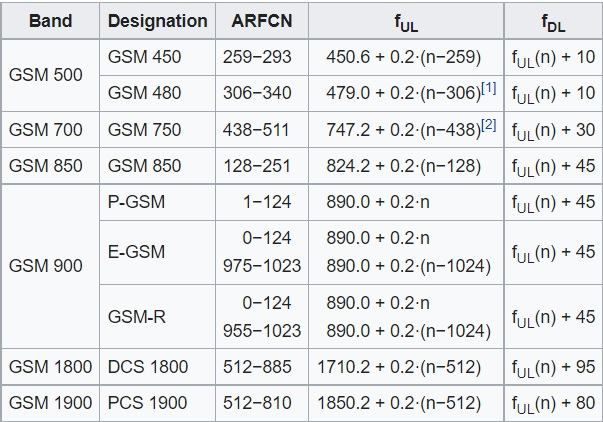
\includegraphics[width=10cm]{Images/ARFCN.jpg}
	\centering
	\caption{\lr{ARFCN}}
	\label{fig:arfcn}
\end{figure}
}
